\subsection{Preparation}
After the initial alignment mentioned by \ref{deny_hamel} up to step 6, in order to see interference fringes one must pre-align the interferometer. This is done by first removing the half-wave plate (HWP)
from the inside of the interferometer.\\
Next, it is importanat to place two irises, one just after the output of the main PBS, and the second one as far away from that one as room on the table will allow.
The reason for this is error propagation. It is much easier to see if the beams are misaligned over a larger distance.\\
Prepare a camera with its lens removed and make sure you can connect and see an image on your computer.\\
Place the camera on the table next to the iris closest to the PBS, make sure the iris is fully open (and the camera pointing the right direction ;) ),
and observe what happens when you change the beams' polarization using a HWP, going from H, to D, to V, and back. If the Sagnac Interferometer (SI) is badly misaligned,
you should be able to see two beams, spatially separated, when rotating the HWP. You may repeat this step for the second iris if you so wish.\\
\subsection{The fun part}
Start with the farthest iris and set the polarization of the pump to either H or V. Here you have to choose which mirrors will be your H mirrors, and which will be your V mirrors.
This is crutial for this to be a time efficient endeavor. It is an arbitrary choice, but one that needs to be made and respected throughout the enterity of the alignment process.
Choose them in an intuitive way for you. Based on \ref{fig:SI}, we choose the H mirrors to be C, and M2, and the V mirrors to be M0, and M1.

\begin{figure}[h!]
\begin{center}
	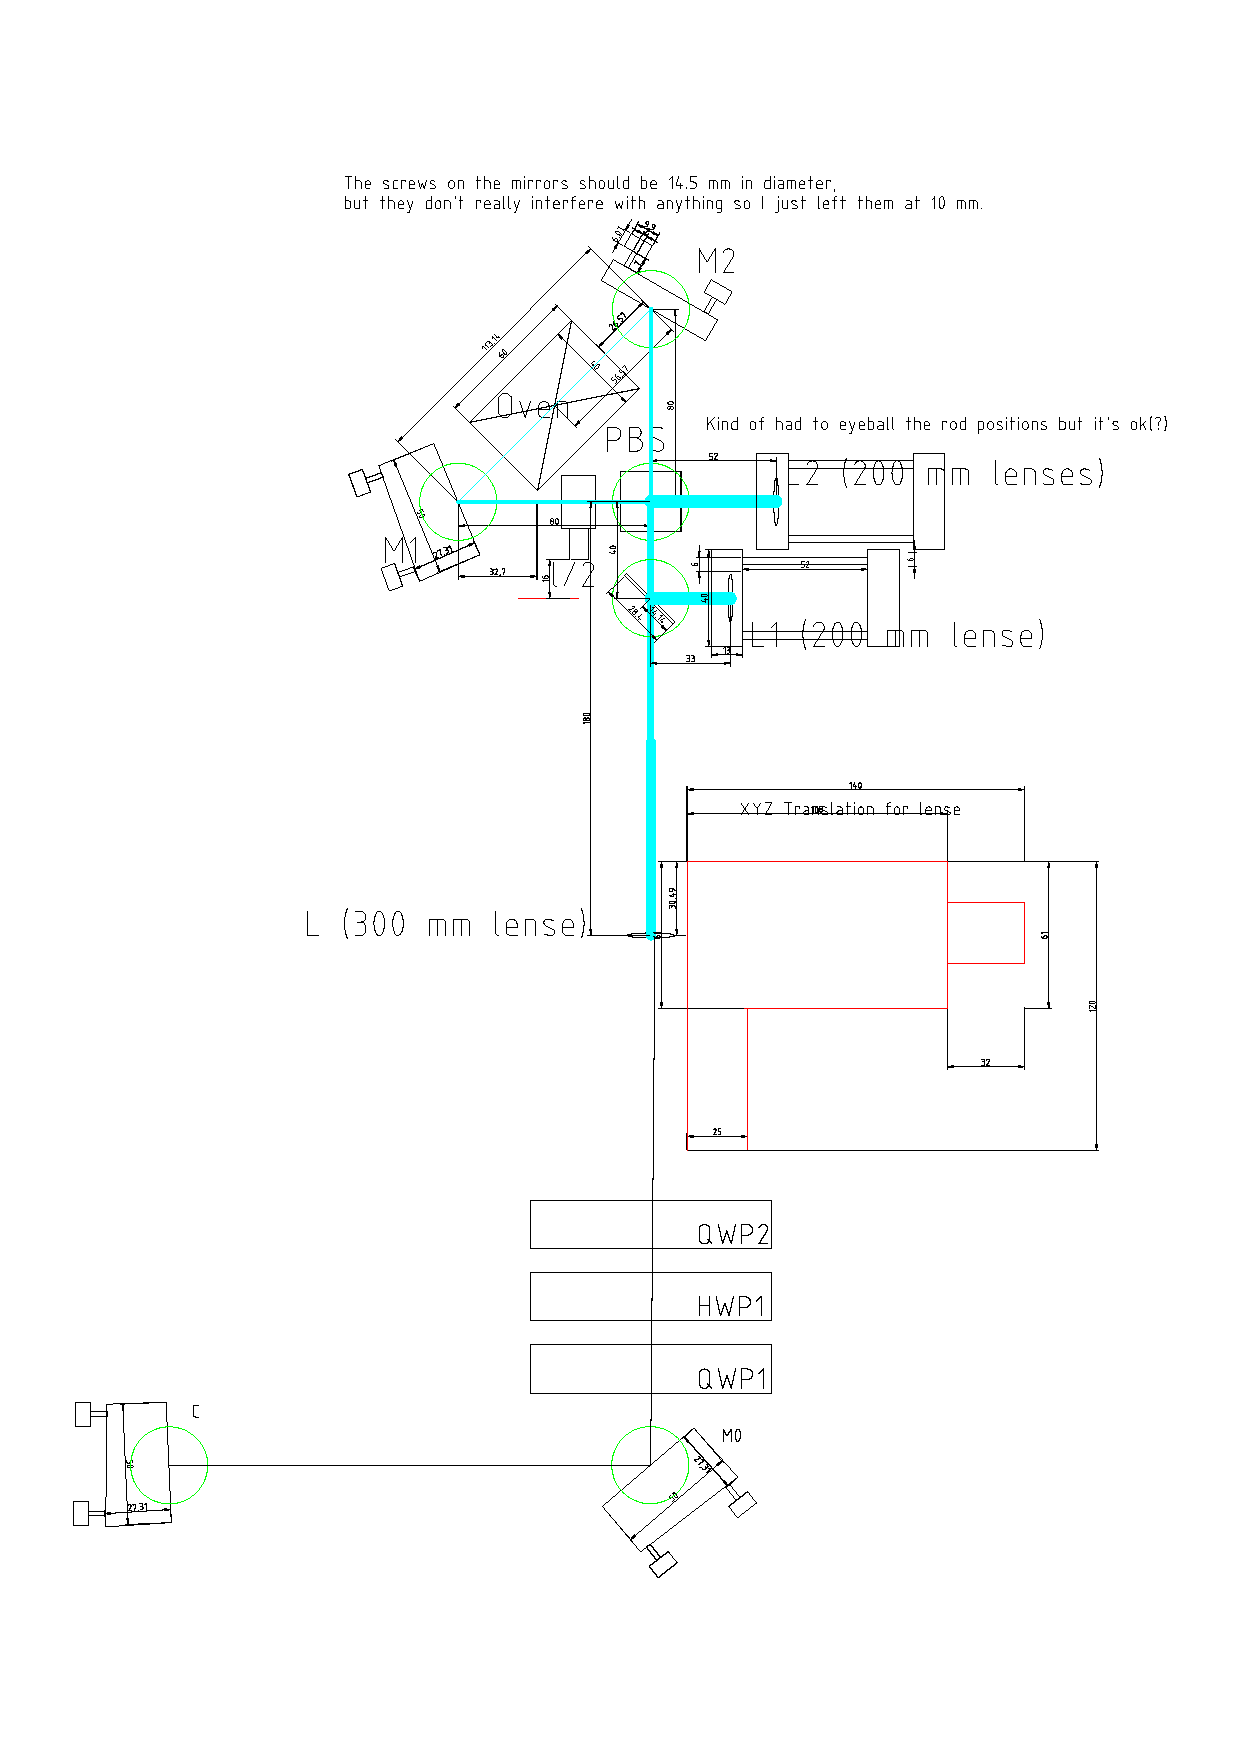
\includegraphics[scale=0.5]{Sagnac_Larger_300mm_Lens.pdf}
\end{center}
\caption{Our SI design}
\label{fig:SI}
\end{figure}

